%03/02 - Miguel Redondo
\chapter{Introducción a la metagenómica}
\section{Importancia de la microbiología}
Los microorganismos desempeñan un papel crucial en la biosfera debido a su participación en el reciclaje de recursos en los ciclos biogeoquímicos y su influencia en eventos histórico-globales, como la primera extinción masiva del planeta ($O_2$). Sólo las cianobacterias son responsables de 1/2 de la actividad fotosintética del planeta (éste -> 🌍).

A nivel aplicado, su relevancia es evidente en campos como: la medicina, por su capacidad patogénica, o la agricultura, donde una problación microbiana (bacterias, hongos, &c.) equilibrada y sana en el (ecosistema que constituye el) suelo es fundamental para el crecimiento saludable de las plantas (como nosotros con los probióticos y los bífidus 👺). La optimización de cultivos agrícolas puede lograrse mediante la modulación de las relaciones microbianas. Lo que permite reducir la dependencia de agroquímicos, cuyo uso excesivo hipersaliniza el suelo, genera toxicidad y contaminan gran parte de los cuerpos acuíferos. 

Los microorganismos también se pueden aplicar en otras tareas como la biorremediación, donde se emplean para restaurar ecosistemas contaminados por hidrocarburos, metales pesados y otros contaminantes. También se explora la producción de biocombustibles a partir de biomasa para reducir la dependencia en los hidrocarburos. Estos ejemplos ilustran solo algunas de las aplicaciones prácticas de la microbiología.

En el cuerpo humano, las bacterias superan $10^1$ en número a las células propias y constituyen aproximadamente 2 kg de biomasa. Estos albergan alrededor de 3.3 millones de genes, distribuidos en más de 1000 spp. de bacterias (estudio de 2010), que exceden por mucho los de nuestro genoma (240K genes). Alteraciones en la microbiota, como el desequilibrio entre \textit{Firmicutes} y \textit{Bacteroidetes}, pueden afectar el metabolismo de nutrientes y contribuir a condiciones como la obesidad, como se ha demostrado en estudios con ratones (🐭). 

Queremos caracterizar e identificar estas comunidades microbianas, sin embargos, caracterizar microorganismos no es sencillo. La aproximación clásica, basada en el cultivo (axénico) y observación microscópica, es limitada, ya que muchas bacterias no son cultivables en laboratorio. Este fenómeno, conocido como la "anomalía del recuento en placa", implica que solo el 15-35\% de la microbiota puede cultivarse (desconocemos sus condiciones de crecimiento o estos son mutalistas obligados). Por lo que no podemos cubrir la diverversidad ni saber todo lo que están haciendo dentro de nuestro organismo. Esto ha llevado al desarrollo de la metagenómica, que permite estudiar comunidades microbianas directamente en su entorno natural sin necesidad de cultivo.

\subsection{Conceptos clave: microbiota, microbioma y metagenoma}
\begin{itemize}
\item \textbf{Microbiota}: Conjunto de microorganismos presentes en un entorno específico (punto de extracción), como el colon o la cavidad bucal, cada uno con una composición característica.
\item \textbf{Microbioma}: Genoma colectivo de una microbiota, es decir, la suma de los genomas de todos los microorganismos presentes. Este término fue acuñado por Hooper y Gordon en 2001.
\item \textbf{Metagenoma}: Técnicas de biología molecular que permiten analizar el microbioma sin necesidad de cultivo. No debe confundirse con el metabarcoding o la metagenómica funcional, que se centran en genes marcadores\footnote{Un gen marcador es un gen que aparece en todos los genomas de una población o en la parte de la población que nos interese, y cuya evolución de cada gen en cada individuo debe permitir discernir a los individuos entre sí. En resumen, debe estar conservado y presentar pequeñas diferencias. Así, se pueden taggear los distintos individuos.} específicos que permiten discernir los distintos individuos en una población. El metagenoma contiene toda la información del microbioma, pudiendo tener acceso a las rutas metabólicas y las condiciones de crecimiento.
\end{itemize}
% Mañana sigo 

La \textbf{metagenómica}, definida en 2005, aplica técnicas genómicas modernas para estudiar comunidades microbianas en su entorno natural, evitando la necesidad de aislar y cultivar especies individuales. De hecho, Wikipedia abarca esa definición, pero comprendiendo también el análisis mediante genes marcadores, pero esto no está estrictamente incluido; la metagenómica es solo para genomas completos, mientras que la secuenciación de amplicones para marcadores específicos.

\section{Genómica vs metagenómica}
La genómica tradicional requiere el aislamiento y amplificación del genoma de organismos individuales, lo que conlleva la pérdida de una gran parte de la población microbiana. En contraste, la metagenómica permite el aislamiento y ensamblaje directo de genomas en contigs, aunque con el riesgo de generar quimeras.

La metagenómica no solo se limita a caracterizar la composición microbiana, sino que también busca entender su funcionalidad. Esto incluye la identificación de rutas metabólicas y actividades enzimáticas, lo que es aplicable tanto a bacterias como a hongos. Para ello, se utilizan técnicas como librerías de expresión metagenómicas y herramientas bioinformáticas como BLAST para buscar genes de interés en contigs ensamblados. No obstante, para ello hay que buscar secuencias concretas de las que se conoce su funcionalidad, pero esto es un proceso lento. Además, algunos organismos pueden haber desarrollado otra secuencia a través de una línea de evolución diferente que tiene una funcionalidad similar, pero que no es conocida.
Los métodos tradicionales, como la PCR y la clonación, son laboriosos y lentos. Hoy en día, las tecnologías ómicas (metagenómica, metatranscriptómica, metaproteómica y metametabolómica) permiten un análisis más rápido y completo de las comunidades microbianas y sus interacciones.

Los procesos en metagenómica son los siguientes:
\begin{enumerate}
\item \textbf{Diseño experimental y muestreo:} Es crucial seleccionar muestras biológicas adecuadas y diseñar experimentos que permitan obtener resultados representativos. Las muestras pueden provenir de agua, suelo o tejidos humanos, y cada tipo requiere protocolos específicos. Por ejemplo, en el caso de una muestra líquida como agua de mar, se pueden utilizar filtros de distinto tamaño, y nos quedamos con el filtro adecuado en función de lo que se desea estudiar.

\begin{figure}[h]
\centering
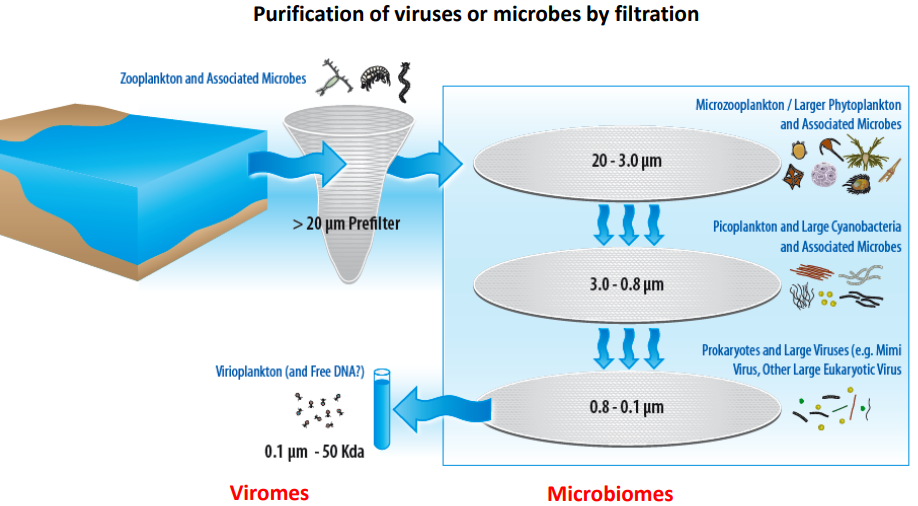
\includegraphics[width = 0.6\textwidth]{figs/filtros.png}
\end{figure}

\item \textbf{Extracción y secuenciación del ADN:} Una vez obtenida la muestra, se extrae el ADN y se prepara para la secuenciación, ya sea mediante fragmentación o amplificación de genes marcadores (como el 16S rRNA).
\item \textbf{Ensamblaje y anotación:} Los fragmentos de ADN se ensamblan en contigs, que luego se comparan con bases de datos para identificar genes y asignar taxonomía. Sin embargo, solo se reconstruye alrededor del 50\% del metagenoma debido a la presencia de genes desconocidos. Además, se utilizan umbrales que descartan contigs de menos de 1000 pares de bases, pudiendo descartar poblaciones minoritarias. Esto se puede salvar utilizando metabarcoding secuenciando un gen (por ejemplo, el gen 16S de la subunidad pequeña del ribosoma) para que las poblaciones minoritarias sí encuentren representación. No obstante, hay que tener en cuenta que con un fragmento tan pequeño no es tan fácil discernir la especie.

\begin{figure}[h]
\centering
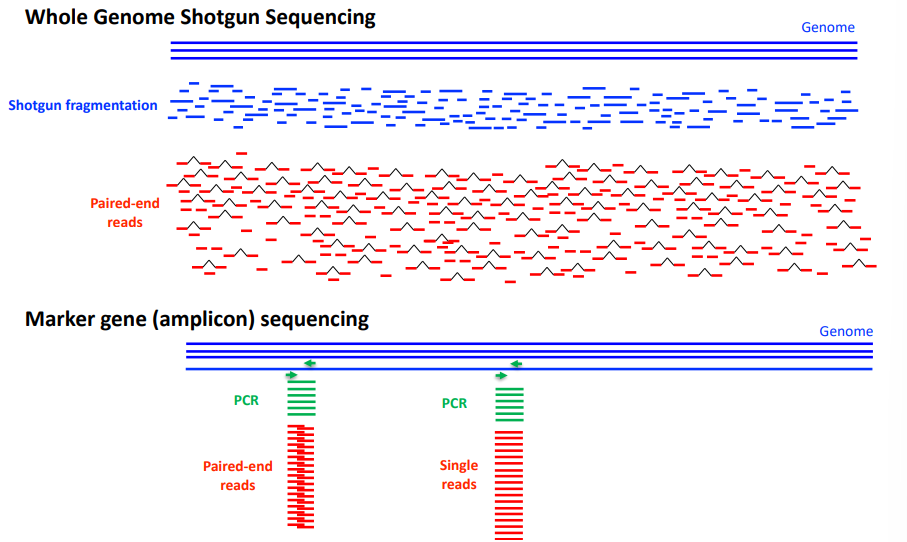
\includegraphics[width = 0.6\textwidth]{figs/assembly.png}
\end{figure}

\item \textbf{Análisis de diversidad y funcional:} Se utilizan herramientas bioinformáticas para analizar la diversidad microbiana y las rutas metabólicas presentes. Esto incluye la creación de perfiles taxonómicos y funcionales. Se ha multiplicado exponencialmente la cantidad de artículos relacionados con el metagenoma y la cantidad de datos en las bases de datos. De hecho, cuando se publican los datos, una de las primeras cosas que piden es subirlo a repositorios como MGnify, MG-Rast, HMP, NCBI-SRA, Metavir, etc.
\end{enumerate}

\begin{figure}[h]
\centering
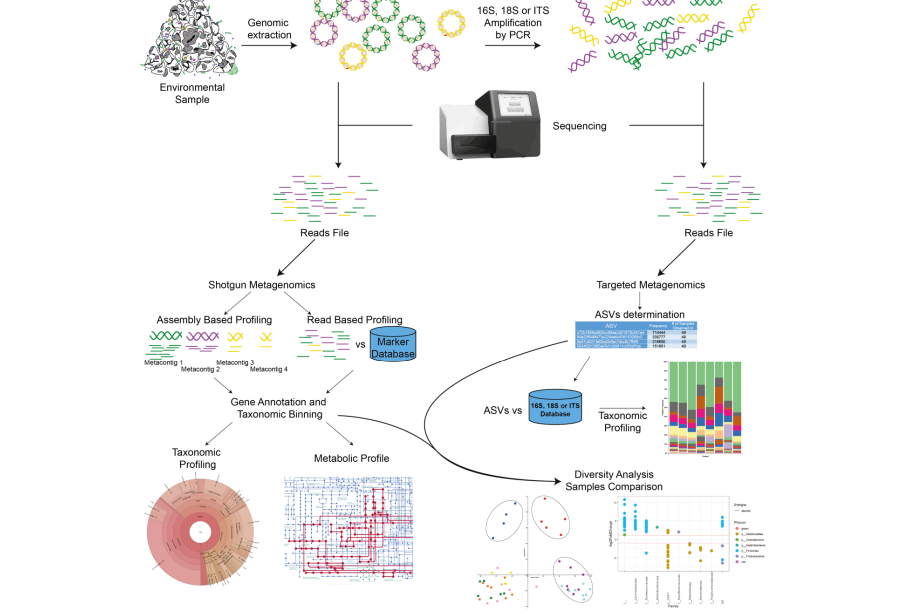
\includegraphics[width = 0.8\textwidth]{figs/metagenomic-pipeline.png}
\end{figure}

\subsection{Ribosoma como reloj evolutivo}
El ribosoma se ha conocido tradicionalmente como el reloj evolutivo, al ser la maquinaria que permite la traducción del ARNm a proteína. Si hay errores en el ribosoma, la mutación es deletérea, al haber una gran presión evolutiva en el ribosoma. Se pueden admitir pequeñas variaciones, las cuales se pueden utilizar para discernir los distintos grupos taxonómicos. 

El ARN ribosomal está presente en todos los organismos vivos, y está conservado al tener un papel crucial. Además, se utiliza para generar un árbol filogenético de todas las especies. Esto sirvió para ver que los ribosomas humanos se parecen más a las arqueas que a las bacterias.

\section{Aplicaciones de la metagenómica}
La metagenómica ha revolucionado el estudio de la microbiota humana y de los ecosistemas. Proyectos como el \textbf{Human Microbiome Project} buscan caracterizar el microbioma humano en diferentes condiciones y localizaciones, identificando correlaciones entre la composición microbiana y enfermedades como la obesidad, la psoriasis y las enfermedades cardiovasculares. A este conjunto de enfermedades se le conoce como \textbf{disbiosis}, patologías causadas por desregulaciones de las poblaciones microbianas. No se conoce si se provoca primero la enfermedad y en base al microclima cambia también la microbiota o al revés, pero la caracterización del microbiota sirve como marcador de estas enfermedades.

Un ejemplo destacado es el tratamiento de infecciones por \textit{Clostridium difficile} mediante trasplantes de microbiota fecal, que han demostrado restaurar la diversidad microbiana y mejorar la salud del paciente. Se utiliza el índice de Shannon como índice de diversidad.

\begin{figure}[h]
\centering
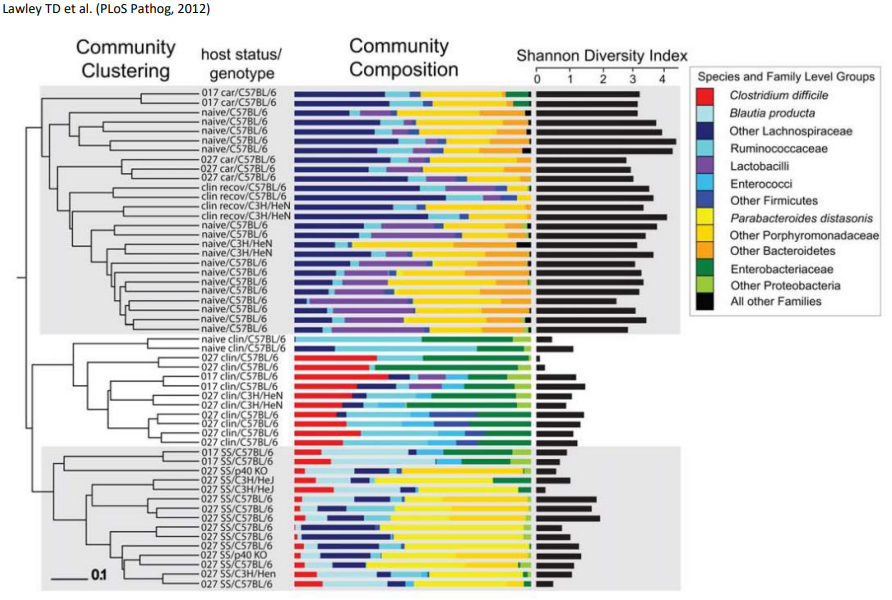
\includegraphics[width = 0.6\textwidth]{figs/c-difficile-1.png}
\end{figure}

\begin{figure}[h]
\centering
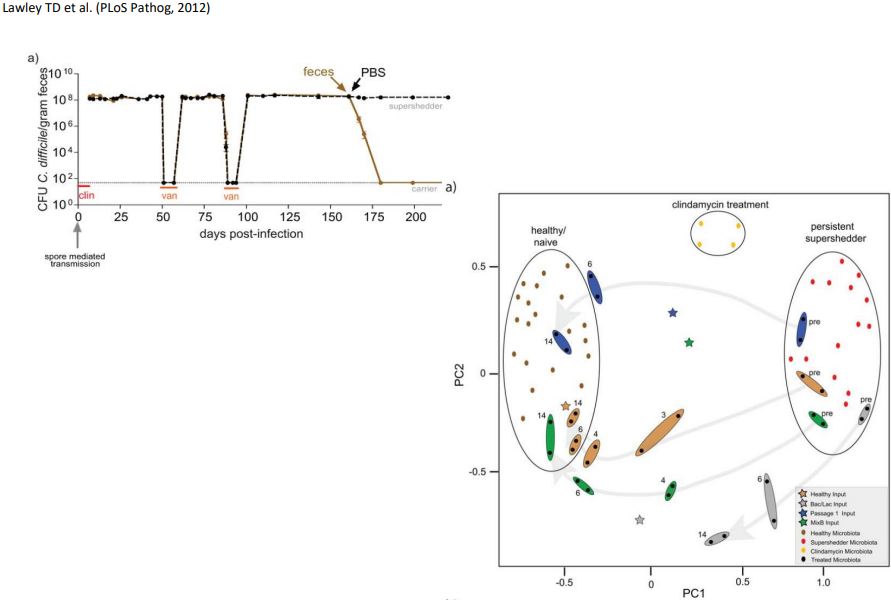
\includegraphics[width = 0.6\textwidth]{figs/c-difficile-2.png}
\end{figure}

\section{Conclusiones}
La metagenómica es una herramienta poderosa para estudiar comunidades microbianas en su entorno natural, superando las limitaciones de los métodos tradicionales. Su aplicación abarca desde la agricultura y la biorremediación hasta la medicina, ofreciendo insights valiosos sobre la diversidad y funcionalidad de los microorganismos. Sin embargo, su éxito depende de un diseño experimental riguroso y del uso adecuado de herramientas bioinformáticas para interpretar los datos generados.
